\section{Experimental Results}\label{sec:results}

\subsection{Experimental Setup}\label{sec:xp_setup}


\begin{figure}[ht!] %FIXME: this figure is not referenced.
  \begin{center}
    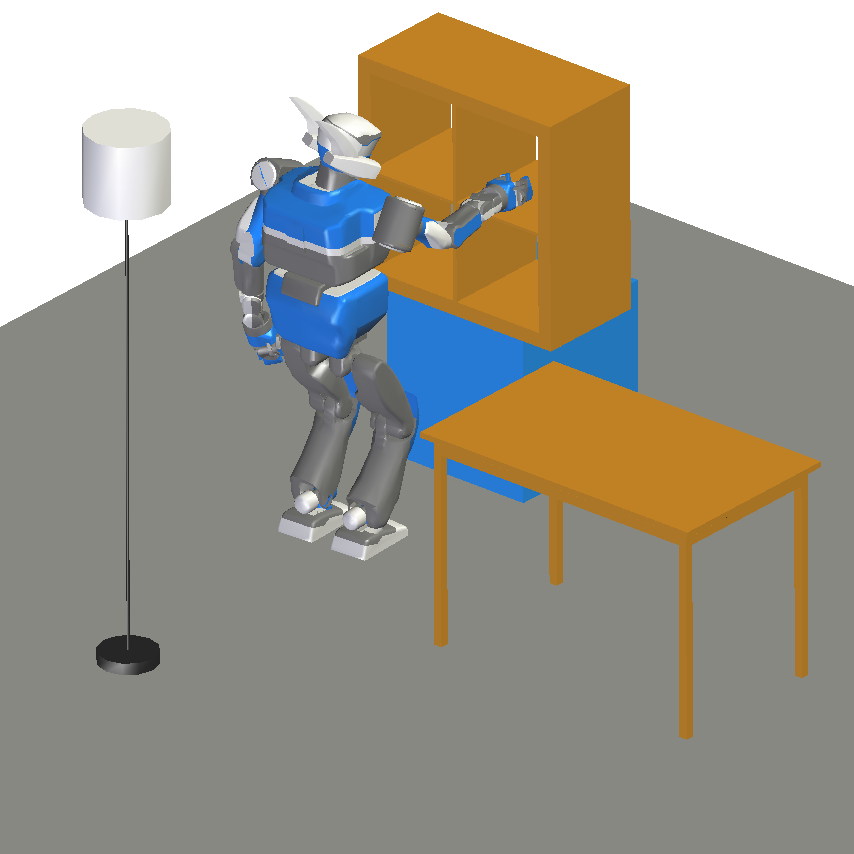
\includegraphics[width=\linewidth]{images/trajectory-8.png}
  \end{center}
  \caption{The HRP-2 robot drops a ball on a shelf while localizing
    itself using vision based localization. \label{fig:xp_setup_screenshot}}
\end{figure}


The experiment demonstrates that by localizing the robot while
walking, HRP-2 can reach a goal position independently of the
execution errors. In the chosen scenario, the robot must drop a ball
on a shelf after walking 2 meters. A more precise description of the
scenario is Fig.~\ref{fig:xp_setup_dim}. Empirically, we estimated the
HRP-2 mean drift to be around one centimeter per step. Considering
that 32 steps are required to reach the goal without hitting the
obstacles, the usual drift would prevent the task from being
accomplished.

\begin{figure}[ht!]
  \begin{center}
    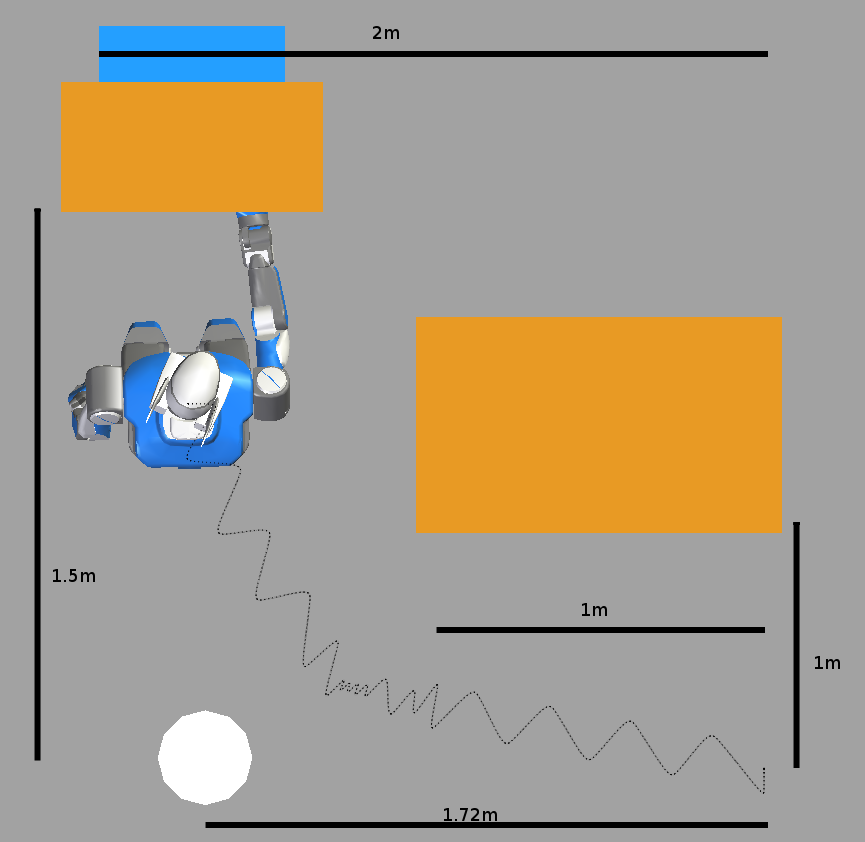
\includegraphics[width=\linewidth]{images/dimensions.png}
  \end{center}
  \caption{Experimental setup description (top view). The dotted line
    displays the robot waist trajectory.\label{fig:xp_setup_dim}}
\end{figure}


The camera trajectory estimated by the localization algorithm is
validated using motion capture data. Markers have been placed on both
the robot head (FIXME and left foot?) to provide ground truth.


Finally, the camera position is given by the algorithm described in
detail in the previous sections. During the experiments, the acquired
image resolution was $320 \times 240$. The localization module has
been running at a mean rate of 16\hertz~during the experiments. The
vision computer running the vision based localization node is a
Intel\textregistered Core\texttrademark\ 2 CPU T7200~@~2.00GHz with
2Gb.\ of RAM.


\subsection{Comparison to Motion Capture Data}\label{sec:mocap}

The Table.~\ref{tab:mocap_comparison} contains the camera position
estimated by the motion capture system and by the localization
algorithm. The mean error is FIXME meters and FIXME rad. Drop in the
algorithm precision can occur when the robot enters a part of the map
which is not dense enough or where the environment does not
incorporate enough texture to detect enough interest points.
%FIXME we will see depending on the final data...


The used motion capture system is a Motion Analysis system relying on
six Eagles and four Hawks cameras. It provides an estimation of the
camera position at 200\hertz~with a precision error of less than one
centimeter.

%FIXME write conclusion -> summarize results.

\begin{figure}[ht!]
  \begin{center}
    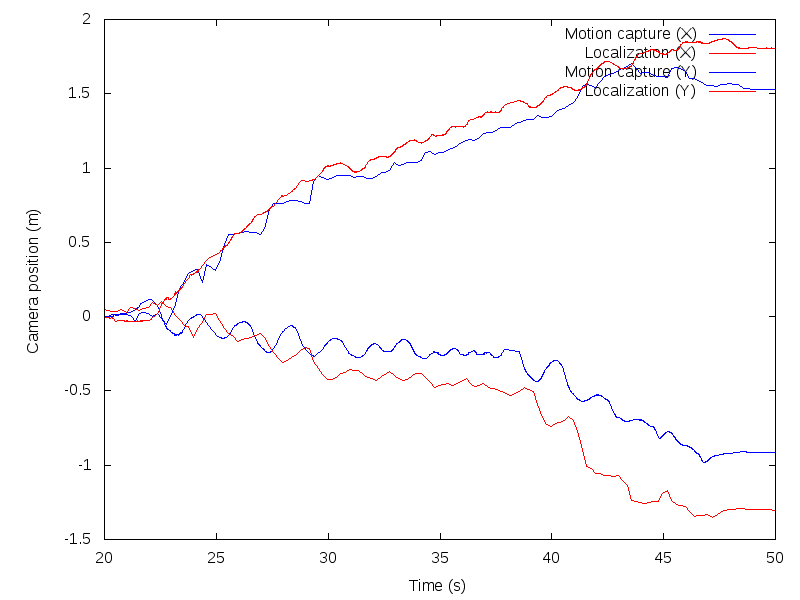
\includegraphics[width=\linewidth]{data/mocap.png}
  \end{center}
  \caption{Camera position estimated by both the motion capture system
    and the localization algorithm. \label{tab:mocap_comparison}}
\end{figure}

\subsection{Timing Evaluation}\label{sec:timing}
\PFA{Here there should be a table for timing evaluation, describing the mean computation times of the vision and control systems}
%%% Local Variables:
%%% ispell-local-dictionary: "american"
%%% LocalWords:  odometry HRP
%%% End:
